\chapter{The Flexible Load: Curtailment and Power Optimization}
\chaptermark{The Flexible Load}
\label{ch:flexload}

Chapter~4 ended with a tripwire: above the breakeven price, a machine is worth more off than on. A tripwire is not an operating strategy. Prices arrive every five minutes, machines pay a real cost for every pause and resume, and the most expensive hours arrive with no warning at all. This chapter builds what actually pulls the trigger: first the power target (a machine's efficiency is not one number but a curve), then \glossaryterm{the-loop}{the loop}, the price-response layer that turns each new price into what the fleet draws, built on exactly three rules, and finally the report card, a benchmark against an oracle that sees the future.

\section{One Point Becomes a Curve}

Everything in Chapter~4 treated a miner as a fixed appliance: a fixed hashrate, power draw and efficiency. That is how stock firmware ships. Modern autotuning firmware removes the assumption: it can hold the machine at any \glossaryterm{power-target}{power target} across a wide range, retuning each hashing chip as it goes, and the single operating point opens into an \glossaryterm{efficiency-curve}{efficiency curve}. Figure~\ref{fig:efficiency-curves} shows two of them, for the two machines of Chapter~4, and their provenance matters: these are not laboratory curves but \emph{fleet averages}, aggregated from the operating data of miners running Braiins~OS in the second quarter of 2026, which this book calls the fleet dataset. % src: Braiins OS fleet telemetry aggregates, quarter 2026-Q2, the author's employer's data; cache analysis/data/miner_efficiency_telemetry_2026q2.csv
Remember which direction is good: efficiency counts the joules spent per unit of hashing work, so a \emph{lower} number means less energy for the same output. Run the S19j~Pro below its stock 3,068~W and its efficiency improves: the fleet average bottoms out at 23.8~J/TH near 1,200~W, against a nameplate of 29.5, because chips run more efficiently at lower voltage and frequency. % src: telemetry cache analysis/data/miner_efficiency_telemetry_2026q2.csv (telemetry refreshed 2026-08-27): best 23.83 J/TH at 1,200 W; nameplate per bitmain2021s19jpro
Push it above stock and it buys extra hashrate at ever-worse efficiency, up to the \glossaryterm{power-ceiling}{power ceiling}, the highest power target the loop will set, here 3,420~W for the S19j~Pro and 3,990~W for the S21~XP. Efficiency, the exchange rate of Chapter~4, turns out to have a throttle attached. % src: ceilings analysis/ch5-backtest/papo_sim.py PARAMETRIC_MINERS p_max 3420 and 3990, kept by telemetry_miner.py build() (its console: floor / default / ceiling 1200 / 3068 / 3420 and 2774 / 3645 / 3990 W), as chapter 9 (analysis/checks/ch9_tuning.R header), below the telemetry extent, 4,400 and 4,600 W; no PSU rating is printed: bitmain2021s19jpro gives none, and bitmain2024s21xp gives an adapted AC output power requirement of 4,000 W (read 2026-09-26, article updated 2026-09-23); Bitmain's PSU pages, read 2026-09-26 through support.bitmain.com/api/v2/help_center/en-us/articles/<id>.json, map the S19j Pro to the APW12 family (15909673875993) and the S21 XP to APW171215a/c or PW380a/b/c (47856379027737), and rate APW12 at up to 240 A at 15 V, 3,600 W (900001205726), and APW171215a at 267 A, at most about 4,005 W at 15 V (32499285460505); so the S19j Pro ceiling sits 5% under its PSU but the S21 XP ceiling only about 0.4% under, and the earlier clause about a margin below the power supply rating is withdrawn

\begin{figure}[h]
  \centering
  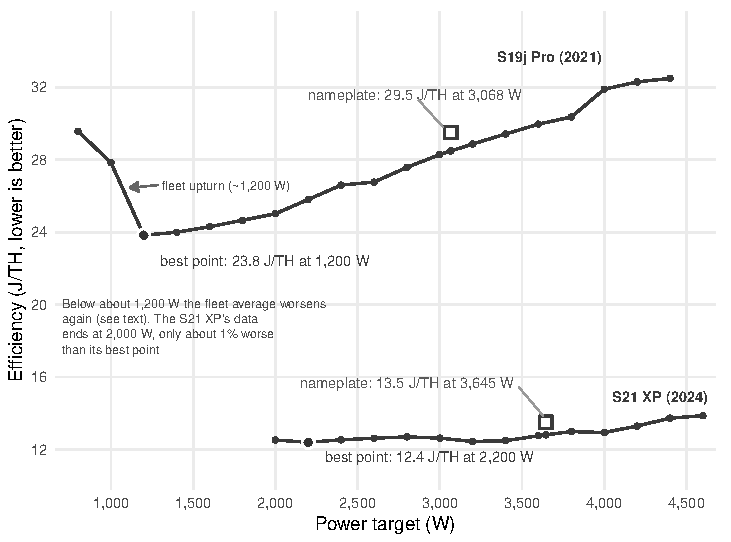
\includegraphics[width=\textwidth]{images/efficiency_curves}
  \caption{
    Measured efficiency curves for the Antminer S19j~Pro and S21~XP: fleet averages of operating data from miners running Braiins~OS, second quarter of 2026. Lower is better. Squares mark the manufacturer nameplate at stock power; filled dots mark each curve's best-efficiency point. The arrow marks where the S19j~Pro's fleet average turns back up, near 1,200~W (see text). The S21~XP's lowest reading, at 2,000~W, is just 1~percent worse than its best point. The loop's power ceilings, 3,420 and 3,990~W, stop short of the curves' right-hand ends; its modulation floors are 1,200~W and, on the S21~XP, Braiins~OS's default minimum, 2,774~W. % fig-src: analysis/figures/fig_ch5_efficiency_curves.R (telemetry cache analysis/data/miner_efficiency_telemetry_2026q2.csv; Braiins data); the modelled V-floor, 1,850 to 1,900 W, is internal Braiins modeling (one engineer's fitted curves, a personal communication) as analysis/checks/ch5_vfloor.py part 2 transcribes it; 1% is analysis/checks/ch5_vfloor.py part 1 (S21 XP 2,000 W +1.03% on the 2,200 W best point); ceilings 3,420 and 3,990 W as the power-ceiling sentence above (analysis/ch5-backtest/papo_sim.py p_max), curves end at 4,400 and 4,600 W; floors 1,200 W (the S19j Pro's best point) and 2,774 W (the S21 XP's Braiins OS default minimum, braiinsacademytechres) as analysis/ch5-backtest/telemetry_miner.py modulation_floor takes them (analysis/checks/ch5_vfloor.py part 3)
  }
  \label{fig:efficiency-curves}
\end{figure}

Two caveats belong to these curves. First, the nameplate is not the field. A machine's rated efficiency is measured on fresh hardware under factory settings; on a real site, every unit differs. Chips vary in quality straight from the fab, the spread miners call the silicon lottery, and machines age: fans wear, thermal interfaces dry out, dust accumulates. The curves here average the machines running Braiins~OS in this dataset; an individual machine sits somewhere around them, not on them. At stock power the autotuned fleet average actually \emph{beats} the nameplate, 28.5 against 29.5~J/TH for the S19j~Pro and 12.8 against 13.5 for the S21~XP, because per-chip tuning recovers headroom that factory firmware, with one setting for every unit, has to leave on the table. % src: telemetry at 3,068 W = 28.48 J/TH (S19j Pro); at 3,645 W = 12.81 vs 13.5 nameplate (S21 XP)

Second, the curve has a bottom, and it is not at zero watts. Below roughly 1,200~W the S19j~Pro's fleet average turns back up. I read such a bottom as the power supply's doing, the \glossaryterm{v-floor}{V-floor}. Modeling work at Braiins supports that mechanism.\footnote{Based on internal modeling work at Braiins.} On the S19j~Pro, at clock speeds of about 300~MHz and below, the hashboards would need less voltage than the supply's minimum output, 12~volts on the APW12 and APW17 supplies Bitmain lists for these machines \autocite{bitmain2025psu}. Past that point only the frequency drops. % src: internal Braiins modeling: Pavel Mikuš, Performance Curves of the Antminer S19j Pro, S21 XP and S21 Pro, personal communication, October 15-16, 2025; Braiins is the author's employer (one engineer's personal communication, internal chat of 15 Oct 2025, on his modelled S19j Pro curve: the sharp break a bit below 2,000 W is where the miner hits the PSU's minimum voltage; at about 300 MHz or below the chips do not need that much voltage, but the PSU cannot go lower, so below the floor only the frequency drops and the extra voltage turns into heat; the 300 MHz is given for the S19j Pro only, no break frequency for the S21 XP or S21 Pro), confirming the mechanism of the author's earlier reading, not the fleet's 1,200 W upturn (the model's break is 650-700 W higher, the reconciliation below), printed as such until 2026-09-26 (STATUS, open item 2); bitmain2025psu (article 15909673875993): S19j Pro on the APW12 (12V-15V) series, S21 and S21 Pro on APW171215a/c or PW380a/b/c under the heading APW17 (12V-15V), PW380; article 47856379027737 gives the S21 XP the same APW171215a/c or PW380a/b/c; the APW12 and APW171215a spec sheets (900001205726, 32499285460505) give OUT1 DC voltage 12V-15V; all four read 2026-09-26 through support.bitmain.com/api/v2/help_center/en-us/articles/<id>.json; PW380 has no published spec, so the 12 V is printed for the APW12 and APW17 only; the upturn itself is in the telemetry cache: S19j Pro 800 W = 29.6 J/TH vs 1,200 W = 23.8 (analysis/checks/ch5_vfloor.py part 1)
The chips then run on more voltage than they need, which forfeits the quadratic voltage saving that made underclocking efficient in the first place: the energy the surplus voltage costs goes into heat, not hashing. Meanwhile the chips' leakage at the pinned voltage, the fans and the control board keep drawing a fixed share, now spread over ever less hashing. Whatever sets a curve's bottom, running below it is strictly worse than running at it: less work \emph{and} worse efficiency. % src: internal Braiins modeling (below the floor the chips run on more voltage than they need, only the frequency drops, and the extra voltage turns into heat); the quadratic voltage saving and the fixed draw (leakage at the pinned voltage, fans, control board) are the author's physics, which the repository does not show beyond one line of arithmetic: the modelled S19j Pro's constant gain below its floor, +2.525 TH/s per 50 W through 73.44 TH/s at 1,850 W, puts about 396 W on a line that does not scale with hashrate, more than fans and a control board draw (analysis/checks/ch5_vfloor.py part 2, an intercept of the quoted line, not a modelled reading); a curve's bottom is its best-efficiency point, below which it has less hashrate and worse J/TH (part 1: S19j Pro 800 and 1,000 W, S21 XP 2,000 W)

The V-floor is a voltage limit, not a fixed wattage; where it falls depends on the type of machine. % src: internal Braiins modeling as transcribed in analysis/checks/ch5_vfloor.py MODELLED (part 2 console): S19j Pro floor about 1,850-1,900 W, 74-76 TH/s (per 50 W step from 1,800 W +2.525, +2.380, +1.293 TH/s; best 25.06 J/TH at 1,900 W; hashrate stops growing at about 5,350 W, 149 TH/s, the PSU's maximum voltage); S21 XP about 1,900-1,950 W, 178 TH/s (a flat +6.685 per 50 W to 1,900 W, then +6.626 and +4.902); S21 Pro about 1,650 W, 122 TH/s (a flat +5.816 to 1,650 W, then +5.14); 1,925 W is the midpoint of the S21 XP's 1,900-1,950 W; the same supply per bitmain2025psu (S21 XP and S21 Pro both APW171215a/c or PW380a/b/c); the caveats are internal Braiins modeling's: a fitted model, a year of telemetry, 42 C average hashboard temperature (which the engineer calls the bosminer default for the model; not the Academy's Default Temperatures, braiinsacademytechres, whose 60 C for the S19J Pro and 65 C for the S21 XP and S21 Pro are target temperatures, a different quantity), errors from Braiins' own power model, not comparable with manufacturer marketing specs

Figure~\ref{fig:efficiency-curves}'s fleet averages do not pinpoint that limit for an individual machine. % src: (2026-10-13, author decision: the prose and the Figure 5.1 caption print only the fleet's 1,200 W, not the modeled single-machine floor of about 1,850-1,900 W, which stays in these notes)  analysis/checks/ch5_vfloor.py part 2 console: S19j Pro fleet at 1,850 and 1,900 W (interpolated) 74.75 and 76.48 TH/s against the model's 73.44 and 75.82 (+1.8%, +0.9%); below the floor the model gains +2.525 TH/s per 50 W, the fleet +1.888 over 1,200-1,800 W (75% of it), and fleet J/TH falls from 24.66 at 1,800 W to 23.83 at 1,200 W (-3.3%); S21 XP fleet best point 2,200 W, 177.47 TH/s (-0.3% on the model's 178); 2,200 W against the model's 1,900-1,950 W is +12.8% to +15.8% (+14.3% on the 1,925 W midpoint); 2,000 W is +1.03% J/TH on 2,200 W and 10.3% below the modelled floor's hashrate; part 1: S21 XP range 12.40-13.87 J/TH over 2,000-4,600 W; the kit's S21 XP floor is not this best point but Braiins OS's default minimum, 2,774 W (analysis/ch5-backtest/telemetry_miner.py modulation_floor, the next paragraph; the retired parametric floor, 2,760 W, runs only under PAPO_PARAMETRIC=1)
% Historical provenance (detail removed from prose on 2026-10-02): the three candidates are the author's reading (2026-09-26), not a finding: the repository cannot test them, because the committed telemetry has no temperature, sample-count or power-source field (analysis/data/miner_efficiency_telemetry_2026q2.csv carries model, power_w, avg_jth and hashrate_ths, and hashrate_ths is power_w / avg_jth); errors from Braiins' power model are internal Braiins modeling's own caveat; the second candidate is braiinsacademytechres, read 2026-09-26: Supported Devices gives the S19J Pro's original PSUs as APW121215a/b/c, and Supported PSU Models gives Power readings: No for APW121215a/b/c (and d/e/f/g), Yes for APW171215a/c, the S21 XP's; Figure 5.1's x axis is the power target, and the CSV's hashrate_ths is power_w / avg_jth
The backtests in this chapter and Chapter~9 use the measured fleet curves. In them the lowest power target is 1,200~W for the S19j~Pro, its best-efficiency point, and 2,774~W for the air-cooled S21~XP, the Braiins~OS default minimum. The latter is a firmware setting, not a claim about the machine's physical limit \autocite{braiinsacademytechres}. % src: braiinsacademytechres, Default Power Limits, read 2026-09-26: Min Power 944 W (S19J Pro, every variant, 2,478 to 3,068 W) and 2,774 W (S21 XP, 3,645 W, 270 TH/s), with 2,316 W for the S21 Pro and Max Power 6,435 W for all three (transcribed in analysis/checks/ch5_vfloor.py ACADEMY); the page warns that pushing a miner to its minimum limit reduces efficiency; analysis/checks/ch5_vfloor.py part 3: 944 W is below the modelled 1,850-1,900 W and 2,774 W above the modelled 1,900-1,950 W; fleet readings below the defaults: S19j Pro 800 W, S21 XP 2,000, 2,200, 2,400 and 2,600 W; the S21 XP's best point, 2,200 W, is part 1 and Figure 5.1; the kit and chapter 9 floor the S21 XP at the default, 2,774 W, the author's decision of 2026-09-26 (analysis/ch5-backtest/telemetry_miner.py modulation_floor and BOS_DEFAULT_MIN_W; analysis/checks/ch9_tuning.R ch9_floor and CH9_BOS_MIN_W; ch5_vfloor.py part 3 console: modulation floor S21 XP 2,774 W, the default minimum, and S19j Pro 1,200 W, the best-efficiency point, its default 944 W being lower), until then at its 2,200 W best point
% Historical provenance (detail removed from prose on 2026-10-02): bitmain2024s21xp (270 TH/s at 3,645 W, rated at inlet air temperature, noise with the fan at max RPM); braiinsacademytechres, re-read 2026-09-27, Default Power Limits: Antminer S21 XP 3,645 W (min 2,774 W, 270 TH/s), S21 XP Imm. 4,050 W (min 2,877 W, 300 TH/s), S21 XP Hyd. 5,280 and 5,676 W (min 3,863 W, 440 and 473 TH/s); analysis/data/miner_efficiency_telemetry_2026q2.csv has model, power_w, avg_jth and hashrate_ths and no cooling field (its S21 XP is the 270 TH machine, analysis/data/README.md)

That throttle, the power target, converts the price signal into something much better than on/off. For any electricity price there is one point on the curve that maximizes profit, which is revenue minus energy cost, and on a linear efficiency model it has a closed-form solution the loop can recompute cheaply. The backtests at the end of this chapter pick the most profitable point on the measured curve itself. Figure~\ref{fig:optimal-power} plots it for the S19j~Pro: cheap hours push the optimum to the power ceiling, expensive hours walk it down the curve, and the walk stops at the \glossaryterm{modulation-floor}{modulation floor}, the lowest power target the loop will set. Those are the two lowest targets given above. Below the S19j~Pro's, slowing down further surrenders more hashrate than the electricity it saves, so no price justifies going there gradually, even though Braiins~OS's default minimum lies lower. The S21~XP's is Braiins~OS's default minimum itself, which sits above that machine's best point. Past the floor there is only one move left, the full pause, and the loop deliberately hands that decision to a different rule with different physics. This gradual repricing of a running machine is \glossaryterm{modulation}{modulation}; the pause is not its job.

\begin{figure}[h]
  \centering
  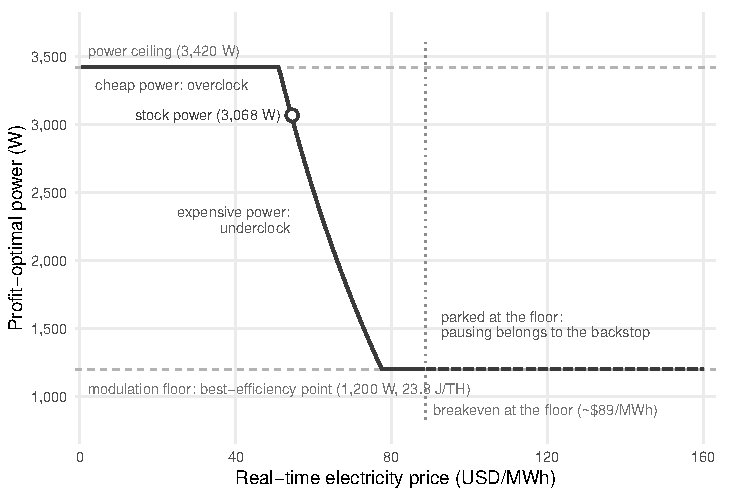
\includegraphics[width=\textwidth]{images/optimal_power}
  \caption{
    What the loop computes: the profit-optimal power level as a function of the real-time price, for the S19j~Pro, using the closed-form solution on its linear-efficiency model fitted to the measured 2026-Q2 curve. Cheap power pushes the machine to its power ceiling; expensive power walks it smoothly down to the modulation floor at the best-efficiency point. Past the floor's breakeven, the target parks (dashed): pausing belongs to the backstop, not to modulation. Hashprice held at its 2025 mean. % fig-src: analysis/figures/fig_ch5_optimal_power.R (closed form per papo_sim.py Miner; anchored to the telemetry's best point and stock value, so figs 5.1/5.2 share one source; optimizing the raw fleet-average spline instead yields artificial steps from averaging lumps -- author caught this 2026-08-28)
  }
  \label{fig:optimal-power}
\end{figure}

\section{Three Facts That Shape the Control Problem}

Designing the reflex around that curve means respecting three facts about the environment it lives in.

First, the price feed is fast, noisy, and mean-reverting. ERCOT publishes a new real-time price every five minutes (Chapter~3); this book borrows the trading floor's word for each published number and calls it a \glossaryterm{print}{print} (ERCOT's own documents call it a Locational Marginal Price, or LMP, and keep settlement point price for the 15-minute price built from those). Five-minute price \emph{changes} are negatively autocorrelated: at LZ\_WEST, from 2024 to mid-2026, the correlation between one change and the next is about $-0.29$. The spikes carry that number. Each of the five largest leaps in the record, all of more than \$4,000, fell straight back at the very next print, so a run-up of that kind predicts a pull-back, not a continuation. Ordinary moves of a few dollars carry almost no signal either way, and in the first half of 2026, when no single print rose by more than \$700, the figure was about zero. % src: analysis/checks/ch5_price_autocorrelation.py, LZ_WEST five-minute prints 2024-01-01..2026-06-22 Central (260,337 change pairs): lag-1 autocorrelation of changes -0.294 (rank/Spearman +0.079); five largest up-moves +4,123 to +4,745, each followed by -4,393 to -4,883; without the 10 largest moves -0.167, without every print above $500 -0.123; by half-year -0.307, -0.266, -0.263, -0.434, +0.020 (2026-H1), with the largest one-print rise +4,431, +4,537, +4,368, +4,745 and +694 (2026-H1 still had 32 prints above $1,000, in runs, not leaps). On the 15-minute settlement series the eight zones run -0.052 to +0.013 (LZ_SOUTH positive), so the figure is a five-minute, spike-driven statistic; the loop decides on the five-minute prints
Whatever the price just did is a bad guide to what it does next; the level, not the trend, carries the information.

Second, wear is real. A fleet that re-applied its optimal target on every print would move about thirty times a day on the S19j~Pro, and about three times on the S21~XP (whose target sits at its power ceiling almost all the time), mostly chasing wiggles worth pennies, and would pause and resume hardware on noise. % src: analysis/ch5-backtest/output/trend_study/sweep_results.csv, persist hold5 (retarget on every print), TEST-2025-26 changes_day 32.0 (S19j Pro) and 2.8 (S21 XP); TUNE-2024 26.9 and 2.9
Moving the target is not always free, and pausing never is. A move to a power target the machine has no saved tuning profile for sends the autotuner walking every chip to new voltage and frequency settings, so the machine hashes below its optimum for the settling period of that tuning run. A target it already holds a profile for can be applied again without a new run, but only that exact target \autocite{braiinsacademyautotuning,braiinsacademydps}. % src: braiinsacademyautotuning, read 2026-09-25 (the hashrate fluctuates noticeably while a machine tunes; once tuning finishes the profile is saved and can be applied again later without waiting for a re-tune); braiinsacademydps, Grid Alignment, re-read 2026-09-26 (with a 3,500 W target and 300 W steps the sequence is 3,200, 2,900, 2,600 and 2,300 W; a start at 66% gives 2,310 W, which is snapped to 2,300 W, since keeping 2,310 would create another sequence of targets that would need to be tuned, slowing the operation and lowering the hashrate); that the reuse holds for the exact target only is also the author's account (2026-09-26); the settling period is the author's round-3 request (2026-08-27), and no duration is printed because Braiins pages disagree on one: about 10 minutes on the Autotuning and About pages, several hours depending on model and control board on the FAQ page (academy.braiins.com/braiins-os/faqs/dps-autotuning), which also says a settled tune can restart after a large change in chip temperature
That cost falls once per target, and the loop uses only a handful.
In this chapter's backtests, once a run has left stock power, it applies only the corner points of its fleet's curve, the targets that can maximize profit as electricity prices change, including the power ceiling: four targets on the S21~XP (2,774, 3,200, 3,400 and 3,990~W) and eight on the S19j~Pro. % src: analysis/ch5-backtest/optimizer_bruteforce_check.py console, re-run 2026-09-26 on the S21 XP's 2,774 W floor: upper concave hull S21XP 2774, 3200, 3400, 3990 W and S19jPro 1200, 1400, 1600, 1800, 2000, 2600, 3400, 3420 W, all on the engine's scan grid (the floor, then every 10 W); the corner points are the hull points, a point no straight line between two others passes above, and the two ceilings, 3,990 and 3,420 W, and the S21 XP's floor, 2,774 W, lie between measured points (3,800 / 4,000, 3,400 / 3,600 and 2,600 / 2,800 W), so they are corners of the curve the engine runs, not measured points; with the floor at the 2,200 W best point the S21 XP's four were 2,200, 3,200, 3,400 and 3,990 W; the claim covers the chapter 5 kit only: its curves (telemetry_miner.py) interpolate hashrate linearly between the measured points of analysis/data/miner_efficiency_telemetry_2026q2.csv and optimal_power() scans them at 10 W from the floor, so profit is piecewise linear in power and peaks on a hull point whatever the price; its "targets the loop applies" block runs every configuration of mixed_basis_study.py at LZ_WEST in TUNE-2024 and TEST-2025-26, 20 runs per fleet, and finds 4 of 4 and 8 of 8 hull points applied, no other target, and stock power only in the 26 intervals per fleet before each run's first move; papo_sim.py simulate() sets the target only to stock power or to an optimal_power() result (or to fixed_power, which only baselines_study.py passes, and only as the power ceiling, a hull point), so every other driver in the kit is bound the same way; chapter 9's engine is not bound to these points: analysis/checks/ch9_tuning.R ch9_curve interpolates J/TH on a 100 W grid and sets hashrate to power / J, which bends between measured points, and ch9_tune and ch9_tune_site may pick any grid point
Each needs one tuning run, unless a large swing in chip temperature restarts it, and every later visit reuses the saved profile \autocite{braiinsacademyautotuning}.
A pause costs more: the machine earns nothing while paused, and although a resume ramps its power back up in about 30 seconds \autocite{braiinsacademyramping}, every full thermal cycle, the boards heating and cooling through tens of degrees, spends a little of the hardware's life. % src: braiinsacademyramping, read 2026-09-27: Quick Ramping, the sequence used when the miner is resuming from a paused state, approximately 30 seconds; ramping also runs in reverse when a miner is paused, for the same time; was "hashing returns within seconds of a resume", per the author 2026-08-28 (a paused machine stays powered); the wear cost is the thermal cycle, not the ramp, which is the author's account
That pause is the firmware's: the machine stops hashing on a pause command but stays powered, its fans still under the firmware's control \autocite{braiinsacademyminerstates,braiinsacademyadvanced}. Opening a breaker, the way Chapter~\ref{ch:ancillary}'s relay-tripped load comes off, is a different act, after which every machine boots, ramps and warms up again. % src: braiinsacademyminerstates, read 2026-09-27 (Mining paused by user: the miner has received a pause command, for example from software used for curtailment); braiinsacademyadvanced, read 2026-09-27 (Control fans PWM after PAUSE: the fans are controlled after the miner enters the PAUSE state, 20% PWM by default, in the GUI's Cooling section since 25.05); that it stays powered is the author's account (2026-08-28) and follows from both; braiinsacademyramping (Normal Ramping, for booting up or restarting, about 30 s, then pre-heating the hashboards, with a timeout of about 10 minutes); chapter-7.tex sec:clr (the under-frequency relay trips the breaker within half a second)
The loop must move only when moving pays.

Third, the stakes are wildly asymmetric. One full-power hour at \$1,600 per megawatt-hour costs an S19j~Pro about 22 times the revenue it earns at 2025's mean hashprice and about 34 times at the lower mean of 2026 to date; for the S21~XP the same hour costs about 10 and 15 times what it earns on those two bases. % src: analysis/checks/ch5_stakes.py section 1: $1,600 / (41,666.7 x mean hashprice / J/TH), on the gap-filled daily hashprice as ch9_hashprice.R builds it; 2025 mean $0.0508/TH/day (365 days), 2026-01-01..08-29 mean $0.0338 (241 days, the window chapter 10 calls 2026 to date); nameplate 29.5 J/TH 22.31x and 33.54x, 13.5 J/TH 10.21x and 15.35x; at the engine's power ceiling on the telemetry curve (3,420 W at 29.47 J/TH, 3,990 W at 12.94 J/TH) 22.29x/33.51x and 9.78x/14.71x, so stock and full power round alike
Such hours are rare but real: LZ\_WEST's settlement point price averaged \$1,600 or more over a full clock hour five times in 2024 and twice in 2025, and the worst hour of 2026 to date, at \$1,330, still cost the S19j~Pro about 28 times what it earned at that period's mean hashprice. % src: analysis/checks/ch5_stakes.py section 2, MIS 13061 LZ_WEST clock hours (Central) whose four intervals average >= $1,600: 5 hours on 3 days (2024), 2 on 2 days (2025, highest $1,905.61 on 2025-01-15 07:00), none 2026-01-01..08-29 (highest $1,329.65 on 2026-01-28 07:00: 27.9x at the period mean hashprice on 29.5 J/TH, the basis of the sentence before; 23.7x at that day's $0.0398); five-minute prints >= $1,600: 54 on 12 days (2024), 22 on 5 days (2025), 0 to 2026-06-22; median five-minute print at or above $1,000: $1,770 (2024), $2,015 (2025)
Missing a spike is catastrophic; a false alarm costs a few minutes of hashing. Any design that treats those two errors symmetrically is wrong.

So the loop has three jobs with three different tempos: follow the price level cheaply and continuously, ignore the noise so hardware survives, and pause decisively when a spike is real. Each job gets its own rule.

\section{One Loop, Three Rules}
\label{sec:threerules}

The loop separates two functions: \emph{modulation reprices the fleet; the} \glossaryterm{backstop}{backstop} \emph{owns pause and resume}. The two mechanisms read the same price feed and never share a decision, which is what keeps noise out of the pause/resume path.

\subsection{Rule 1: Follow the Level}

Every five minutes, the loop recomputes the profit-optimal power target of Figure~\ref{fig:optimal-power} from the newest print, unmodified. Using the last print as the decision price is called \glossaryterm{persistence}{persistence}, and it is a measured choice; the case against forecasting comes below. The target is clamped between the modulation floor and the power ceiling. A print is already in force before anyone outside ERCOT can read it. ERCOT stamps each price with the moment it takes effect and publishes it straight after the SCED run that sets it \autocite{ercot2026protocols}: the posting lands a median 22 seconds after the five-minute boundary. % src: analysis/checks/ch5_posting_latency.py console, on ERCOT's public MIS listing of NP6-788 (reportTypeId 12300) as snapshotted by analysis/data/fetch_ercot_np6788_posting.py: 1,569 on-cycle SCED runs 2026-09-20..25 Central (5.4 days, 0 missing windows), posted median 22 s / p95 28 s after the five-minute boundary, SCED stamp median 19 s after it; ercot2026protocols sec. 6.3.2(2): LMPs posted immediately subsequent to deployment of Base Points and Ancillary Service awards from SCED, with the time stamp the prices are effective; the print stamped b prices [b, b+5) at zero lag (analysis/ch5-backtest/ingest/verify_alignment.py); when a posted print becomes readable is not measured (a listing probe timed a CDN cache, not ERCOT, and was withdrawn 2026-09-25)
Reading it takes longer. Polled through ERCOT's public API every 20 seconds for ten days in autumn 2026, a print became readable a median 2.9~minutes after its boundary, and 3.5~minutes in the evening hours, so more than half of its own interval is gone before the loop can act on it. % src: analysis/checks/ch5_api_readability.py console, on analysis/data/ercot_api_readability_polls.csv.gz (37,780 polls 2026-09-25 02:11 to 2026-10-05 02:11 Central, written by analysis/data/ercot_api_readability/poll.py, one poll every 20 s, arrival timed at the midpoint between successful polls): NP6-788 full window n=2,448 on-cycle prints, median 172.0 s after the five-minute boundary (2.87 min), p95 296.0 s; 18:00-22:00 Central median 212.0 s (3.53 min), other hours 169.0 s; the clean window without the 2026-09-30..10-02 connection outage gives a median of 171.0 s
The backtests assume a full interval of delay before the loop sees each print, which covered 95~percent of the prints polled; in them it is always steering on the most recent past, never the present. % src: analysis/checks/ch5_api_readability.py console, "readable within one five-minute interval of its boundary: 2332 of 2448 = 95.3%"; the other 4.7% (116) arrived later, max 887 s

\subsection{Rule 2: Ignore the Noise}

Computing a target every five minutes does not mean applying it every five minutes. By default the applied target holds for 30 minutes. A plain hold has a flaw, though: when the price gaps to a new level, the fleet can run up to 25 minutes on a stale target. The fix is the \glossaryterm{price-deadband}{price deadband}, one extra condition on the hold: re-apply immediately whenever the newly computed ideal target diverges from the applied one by more than 10~percent of the machine's stock power. Figure~\ref{fig:deadband} shows the two behaviors on one trace. In the calm stretches the price deadband never fires and the wear profile is identical to the plain hold; each time the price gaps, up and then back down, it fires once, and the fleet reprices within five minutes instead of thirty. % src: analysis/figures/fig_ch5_deadband.R console: deadband fires 2 times, at 80 and 135 min, on the gaps at 75 and 130 min; largest ideal-vs-applied gap in the calm stretches 116 W against a 307 W deadband

\begin{figure}[htbp]
  \centering
  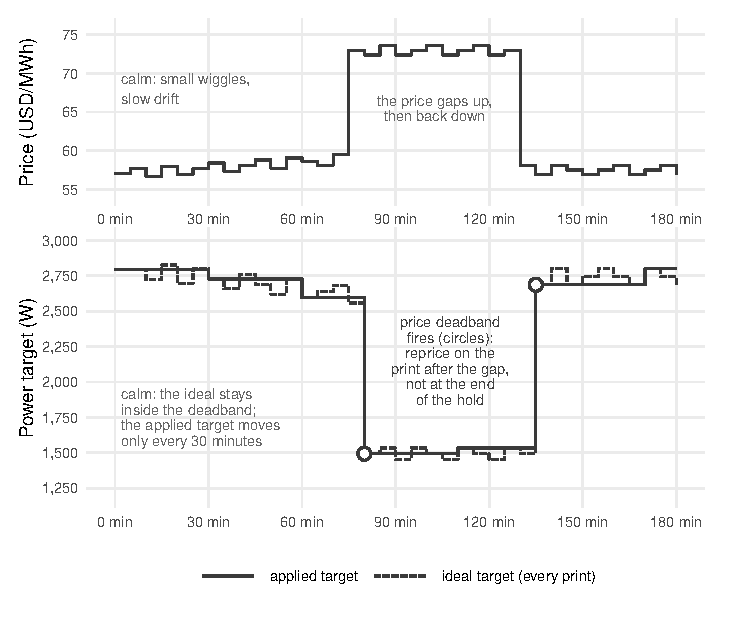
\includegraphics[width=\textwidth]{images/deadband}
  \caption{
    The 30-minute hold and the price deadband that breaks it, on an illustrative price trace, for the S19j~Pro on the same model and optimizer as Figure~\ref{fig:optimal-power}. Through the calm stretches the ideal target (dashed) wiggles inside the price deadband, so the applied target (solid) moves only on the routine 30-minute cadence. When the price gaps up, and again when it gaps back down, the ideal diverges by more than 10~percent of stock power, the price deadband fires (circles), and the fleet reprices on the next print instead of waiting out the hold. Each price print is seen one interval late. % fig-src: analysis/figures/fig_ch5_deadband.R (illustrative trace; measured constants: 30-min hold, deadband 10% of 3,068 W = 307 W, each print seen one interval late; linear-efficiency model anchored at the telemetry's 1,200 W best point and at stock, as fig 5.2; console: fires 2 times, at 80 and 135 min)
  }
  \label{fig:deadband}
\end{figure}

On the older fleet the price deadband is worth real money, and it is not free. In the out-of-sample backtest at the end of this chapter, it adds 2.6~percent to what the plain hold earns over running at stock power on the S19j~Pro fleet, for about 26 target moves a day against the hold's 13. The S21~XP's flat curve leaves it less to do: 0.5~percent more, at under three moves a day. % src: analysis/ch5-backtest/output/trend_study/mixed_basis.csv, TEST-2025-26, LZ_WEST, 5-minute feed, plain hold (decide-5 S14) vs deadband 10% (decide-5 +deadband10): vs_basis_s14 +2.5559 (S19j Pro) and +0.4723 (S21 XP), the deadband's gain as a share of the plain hold's gain over stock power; pct_of_s1 93.85 -> 96.25 and 97.61 -> 98.07; changes_day 13.4 -> 26.3 and 1.6 -> 2.4; on the S21 XP's 2,774 W floor (+0.7535, 2.6 moves a day, on its 2,200 W best point until 2026-09-26)
The backtest charges nothing for a move, so both gains are counted before whatever the extra moves cost on a given fleet's firmware. % src: analysis/ch5-backtest/papo_sim.py simulate(): once the hold or the price deadband allows it, applied = ideal within the same interval and profit is booked at full curve efficiency, with no per-move charge (changes counts the moves and nothing else)
The price deadband is also a dial rather than a knife-edge on the S19j~Pro: widening it to 25~percent keeps about four-fifths of the benefit while cutting the extra moves roughly in half, which makes it the one knob worth handing an operator with a wear budget. The S21~XP has little to trade: at 25~percent its extra moves, under one a day, all but vanish, and it keeps under a quarter of the benefit. % src: analysis/ch5-backtest/mixed_basis_study.py console "dial" lines, TEST-2025-26: deadband25 keeps 82% (S19j Pro) and 23% (S21 XP) of deadband10's gain over the plain hold, at +6.0 and +0.0 moves/day above the hold against +12.9 and +0.8 for deadband10 (changes_day 1.6 for both the S21 XP's plain hold and deadband25); in the 2024 tuning year it keeps 93% and 19%; on the S21 XP's 2,200 W best point, its floor until 2026-09-26, the S21 XP kept 64% (2024: 65%) at +0.5 against +1.0

\subsection{Rule 3: Survive the Spikes}

Pausing hardware is expensive, and five-minute prices mean-revert, so the backstop does not pause just because a print crosses breakeven. It reacts to \emph{accumulated damage}. While the price sits above the machine's breakeven at its most efficient power target within the loop's operating range (on the S21~XP 3,200~W, above its floor), the excess integrates: each print adds its excess over breakeven multiplied by the time it covers, which is what one megawatt at that target loses at that price. The moment the total reaches \$10 per megawatt, the fleet pauses. % src: analysis/ch5-backtest/papo_sim.py K_TRIP = 10.0 ($ per MW), applied in simulate(): while running, area += (p_prev - be_val) * dt_h when p_prev >= be_val and area = 0 when p_prev < be_val, pause once area >= K_TRIP (subject to MIN_UP_S and MAX_CYCLES_DAY); $/MWh x h = $ per MW of load; be_val = breakeven_best(hashprice) of the engine miner, in the default telemetry mode analysis/ch5-backtest/telemetry_miner.py TelemetryMiner.breakeven_best (best breakeven over the engine's power range, floor to ceiling: at 1,200 W on the S19j Pro, its modulation floor, and at 3,200 W on the S21 XP, above its 2,774 W floor; papo_sim.py check_breakevens pins 77 and 148 $/MWh at $44.31/PH/day), recomputed each UTC day; papo_sim.py Miner.breakeven_best applies only under PAPO_PARAMETRIC=1; every chapter 5 driver imports this simulate()
A shallow blip never trips it, because the integral resets when the price dips back below breakeven. A sustained spike trips it fast, and the worse the price, the faster the trip: a single print \$120 or more above breakeven carries \$10 per megawatt in its five minutes and trips it on its own. Figure~\ref{fig:backstop} traces one full pause-and-resume cycle. % src: analysis/figures/fig_ch5_backstop.R console, one print trips on its own at $120/MWh above breakeven (five-minute print) or $40 (15-minute print): K_TRIP $10 per MW over 5/60 h and 15/60 h; the five-minute case is the mixed-basis backtests (sec=300), the 15-minute one multizone_study.py (sec=900); a trip also needs 30 minutes since the last resume and a cycle left in the day (papo_sim.py simulate())

\begin{figure}[htbp]
  \centering
  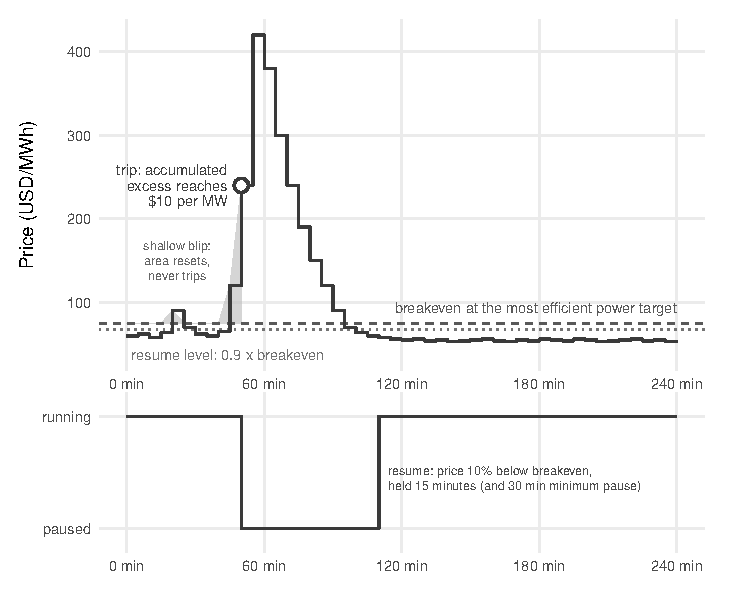
\includegraphics[width=\textwidth]{images/backstop}
  \caption{
    One backstop cycle, on an illustrative price trace. The shaded area is the trip statistic: price excess above the breakeven at the most efficient power target, integrated over time, reset whenever the price dips back below breakeven. Only sustained or very tall spikes pause the fleet. The trip, resume and minimum-time constants are the ones the backtests use. % fig-src: analysis/figures/fig_ch5_backstop.R (illustrative trace drawn with no feed lag; trip, resume and minimum-pause constants as analysis/ch5-backtest/papo_sim.py K_TRIP, RESTART_BAND, DWELL_S, MIN_DOWN_S, resuming on the third calm print as the kit does; console: trip at 50 min, restart at 110 min)
  }
  \label{fig:backstop}
\end{figure}

Resuming is deliberately asymmetric: the price must fall to 10~percent below breakeven and hold there for 15 minutes before the fleet comes back, and minimum runtimes of 30 minutes in each direction plus a budget of at most eight cycles per day cap the worst case. % src: analysis/ch5-backtest/papo_sim.py backstop constants, applied in simulate(): RESTART_BAND = 0.10 (resume needs p_prev <= be_val * 0.90), DWELL_S = 15*60 (held for 15 minutes of prints: three five-minute prints or one 15-minute print, t_prev - calm_since >= DWELL_S - sec), MIN_DOWN_S = MIN_UP_S = 30*60 (no resume within 30 min of a pause, no pause within 30 min of a resume), MAX_CYCLES_DAY = 8 (pauses per UTC calendar day; resumes are not budgeted, a detail left out of print per author 2026-08-28)
In thirty months of backtest across all eight ERCOT load zones the backstop tripped 0.12 to 0.53 times per day depending on the fleet and the zone, and adding the price deadband changed that count by exactly zero in every zone: modulation and pausing stay fully decoupled, as designed. % src: analysis/ch5-backtest/multizone_study.py summary (output/trend_study/multizone_rtm15.csv; 15-minute settlement prices, 2024-01-01 to 2026-06-23 UTC, 8 zones x 2 fleets): plain-hold backstop pauses 0.12 to 0.53 per day across the 16 cells and both windows; change in the pause COUNT with the deadband 0 in all 16 cells at every width from 10 to 40%, both windows

\section{Why There Is No Forecast}

The chapter's backtests compared sixty-seven alternatives to the last print, spanning slope extrapolation over 10-to-60-minute windows, exponential smoothing, rolling quantiles, and constant risk biases, and out of sample none of them beat it by anything worth building. On the S19j~Pro fleet nothing beat it at all; on the S21~XP three smoothing and rolling-quantile variants edged ahead by at most 0.2~percent of the plain hold's gain, under a dollar per machine in eighteen months. Across all eight load zones on the settlement point price, only the two gentlest slope settings, which barely extrapolate, came out ahead, by at most 0.12 percent; every other signal tested there lost in all sixteen zone-and-fleet combinations. % src: analysis/ch5-backtest/reactive_papo_trend.py summary (output/trend_study/sweep_results.csv; LZ_WEST five-minute prints, 30-minute hold, 67 signals plus persistence): TEST-2025-26 S19j Pro 0 of 67 beat persistence (best slope-ols W60 g5 -0.19% of the hold's uplift); S21 XP 3 of 67, ewma hl10 +0.16%, quant W15 q60 +0.13%, ewma hl15 +0.10% (counted on delta_pct; the summary once tested whole-dollar delta_vs_s14 and dropped wins under $0.50) (delta_vs_s14 $1, $1, $1 per machine over 538 days, whole dollars; ewma hl10's 0.16% of the hold's $542 uplift is about $0.87); on the S21 XP's 2,200 W best-point floor, until 2026-09-26, 5 of 67, best ewma hl10 +0.29%, about $1.57; no slope extrapolation beat it on either fleet; in sample (TUNE-2024) 6 and 9 smoothing or quantile variants did (6 on the S19j Pro in the committed CSV before and after the floor change; this comment said 5 until 2026-09-26). multizone_study.py summary (multizone_rtm15.csv), 7 representative signals: out of sample some signal beats persistence in 10 of 16 cells, only slope-ols W30 g5 and W60 g5, best +0.12%; the other five lose in all 16 (8 of 16 on the S21 XP's 2,200 W best-point floor, until 2026-09-26); in sample (TUNE-2024) bias +$10 also edges ahead in one cell, LZ_CPS S21 XP, by $0.06 (+0.01%), on the 2,774 W floor (behind in every cell on the 2,200 W one), hence no "ever" in the prose
The reason is structural, not a matter of tuning: because a big five-minute leap upward usually falls straight back, extrapolating a trend points the decision in exactly the wrong direction, and it is most wrong during spikes, when the stakes are highest.
Leaning the other way does little better. Out of sample, none of the six variants that push the decision price against every recent move beat the last print by more than 0.15 percent of the plain hold's gain, under a dollar per machine in eighteen months, and the two that push against falls but not rises, one of them extrapolating rises instead, lost on both fleets. On the 15-minute settlement point price in the eight load zones, none came out ahead at all. % src: analysis/ch5-backtest/fade_study.py --summary-only (output/trend_study/fade_study.csv; the eight fade signals of trend_followup.py EXTRA, decision price = last print + g x recent slope with g < 0, plain 30-min hold, delay 1, wins counted on the dollar delta to the cent): TEST-2025-26 LZ_WEST five-minute prints, rows equal to followup.csv; the six that fade every move (fade-end W15 and W30 at g -5 and -10, fade-ols W15 g-5, fade-ols W30 g-10) best fade-end W15 g-5 +0.15% of the hold's uplift, $0.81 per machine over 538 days (S21 XP), and fade-end W30 g-5 +0.15%, $0.50 (S19j Pro); the two fade-asym signals fade falls only (up0 dn-10) or fade falls and extrapolate rises (up15 dn-10), -0.22% and -1.90% (S21 XP), -0.64% and -2.72% (S19j Pro); deciding on the print and billing on the settlement point price at LZ_WEST, best +0.15% ($0.82) and +0.15% ($0.52); 15-minute settlement point price, 8 zones x 2 fleets, ahead in 0 of 16 cells, best -0.00% (-$0.02, fade-end W15 g-5, LZ_WEST S21 XP); on the S21 XP's 2,200 W best-point floor, until 2026-09-26, the S21 XP's best was +0.32% ($1.71) and 1 of 16 cells came out ahead by $0.02; worst -1.78% (-$3.81, fade-end W15 g-10, LZ_HOUSTON S19j Pro), largest dollar loss -$4.69 (-1.37%, same signal, LZ_WEST S19j Pro); at 15 minutes the W15 OLS-based signals, both fade-asym among them, equal persistence (two prices in the window) and fade-ols W30 g-10 equals fade-end W30 g-10 (three equally spaced prices), so four distinct signals are scored there; in sample (TUNE-2024) 6 of 8 on both fleets at five minutes, best +0.41% and +1.00%, 3 of 16 settlement cells, best +0.25%; two probes that fade rises only, not among the eight, best +0.31% ($1.71, S21 XP, five-minute prints), both lose on the S19j Pro, at most +0.08% in 7 of 16 settlement cells
These tests support persistence over the self-built signals tried here. They do not settle the make-or-buy question: no commercial forecast feed was tested. A paid feed would have to improve the loop's realized margin after its fee and the site's operating constraints, not merely predict prices more accurately.

\section{Two Prices, One Decision}

Chapter~3 left a subtlety that this loop has to respect: ERCOT bills a site on the 15-minute settlement point price, but publishes a fresh five-minute price three times per settlement interval. The loop decides on the five-minute print. Consumption is continuous, so a reaction to an interval's first print still changes the power drawn over the rest of that interval; the backtests, which let each print act only once its own five minutes are over, give it at most the remaining two-thirds. % src: arithmetic: SCED prices about every five minutes against 15-minute settlement intervals (ercot2026rtm), the settlement point price built from the interval's SCED LMPs (ercot2026protocols sec. 6.6.1), so three prints per interval; analysis/ch5-backtest/papo_sim.py load_mixed_basis bills each five-minute sub-interval at its interval's settlement point price, and simulate(delay=1) runs sub-interval i on print i-1, so the target set on the first print applies from the second sub-interval and carries into the third unless the second print moves it (mixed_basis_study.py docstring)
The catch the backtests exposed is that the fast feed and the price deadband work best together: under a plain 30-minute hold, five-sixths of the fresher prints arrive when the loop is not allowed to act. The fast feed alone adds little to what the plain hold earns over stock power (0.4~percent on the S21~XP fleet out of sample and 1.1~percent on the S19j~Pro; in 2024, the year that set the price deadband's width, it cost the S21~XP 0.8~percent). Together the two are worth more than the sum of their parts in all four window-and-fleet combinations the companion repository runs at LZ\_WEST. % src: analysis/ch5-backtest/output/trend_study/mixed_basis.csv, LZ_WEST, pct_of_s1 (capture) and vs_decide15_s14: TEST-2025-26 fast feed alone (decide-5 S14) 97.61 vs 97.23 (S21 XP), 93.85 vs 92.85 (S19j Pro), +0.38% / +1.07%; deadband alone (decide-15 +deadband10) +0.25% / +1.78%; together (decide-5 +deadband10) +0.86% / +3.66%. TUNE-2024 fast feed alone 94.34 vs 95.09 (S21 XP, -0.78%) and +1.06% (S19j Pro); deadband alone +0.31% / +2.35%; together +0.02% / +4.94%. Together exceeds the sum of the two alone in 4/4 cells
Speed pays on its own terms, too: every extra five minutes of feed latency costs the full loop about 0.8~percent of its gain over stock power on the S21~XP and 1.7~percent on the S19j~Pro, and a second five minutes costs about as much again, which makes fast ingestion part of the algorithm. % src: mixed_basis.csv TEST-2025-26 LZ_WEST, vs_full_loop of the full loop with one and two extra intervals of delay: decide-5 +deadband10 delay2 -0.76 (S21 XP) and -1.74 (S19j Pro); delay3 -1.48 and -3.66

One more reason the settlement point price matters: the adders. From half past five to a quarter past eight on the morning of January 13, 2025, LZ\_WEST's five-minute prints stayed below \$78, yet the settlement point price billed for those intervals reached \$187.77, 2.6 times the highest print in its interval; the difference was the reserve-scarcity adders of Chapter~3 riding on top. % src: analysis/checks/ch5_adder_example.py (LZ_WEST; MIS 13061 settlement vs NP6-788 prints): 2025-01-13 07:15 Central settled $187.77 on prints $71.16, $64.51, $71.62 (2.62x the highest); an unbroken run of 7 intervals, 06:30 to 08:15 Central, settled $115.59 to $187.77 while no print from 05:30 to the run's last, 08:10, exceeded $77.68 (the day's next print above it, $84.12, came at 17:35 Central). Replaces the $1,629.89 of 2025-06-30, a corrupted row of the legacy cache (ERCOT's archive has $34.17)
A loop deciding on bare five-minute prints would have hashed straight through. On that day's hashprice an S19j~Pro loses money above \$96 even at its most efficient point, so for an hour and three-quarters an S19j~Pro fleet ran at a loss that no print revealed. % src: ch5_adder_example.py: hashprice $0.0550/TH/day on 2025-01-13 (analysis/data/hashprice_daily.csv); S19j Pro best-point breakeven $96.21 (41,666.7 x hashprice / 23.83 J/TH), stock $77.72; every print below it and every settlement of the run above it. For the S21 XP (breakeven $184.27 at its most efficient power target, 3,200 W, 12.44 J/TH, the best efficiency in the loop's range; $184.95 at its 2,200 W best point, the floor until 2026-09-26) only 1 of the 7 intervals settled above breakeven, so the claim is made for the S19j Pro
The reliability-deployment adder adjusts prices for the effect of ERCOT's interventions to keep the grid reliable. The example predates RTC+B, which on December 5, 2025 retired the ORDC adder and moved scarcity pricing into the energy price itself (Section~\ref{sec:rtcb}); the reliability-deployment adder remains, so the bill can still run ahead of the prints: on March 23, 2026, LZ\_WEST settled at \$950.48 in an interval whose highest print was \$758.06 \autocite{ercot2025rtcblive,potomac2026somercot,ercot2026protocols}. % src: analysis/checks/ch5_adder_example.py console, "largest settlement above the highest print after RTC+B: 2026-03-23 21:45 Central, settled $950.48 on a highest print of $758.06" % src: ercot2025rtcblive (go-live Dec 5, 2025); potomac2026somercot p. 2 (ORDC adder "discontinued in December 2025 with the introduction of RTC"; shortage pricing "incorporated into the price of energy rather than functioning as a separate adder"), as chapter-3 sec:rtcb; ercot2026protocols sec. 6.6.1 (current Real-Time Settlement Point Price includes the reliability-deployment adder). ch5_adder_example.py: LZ_WEST intervals settled at $100 or more and above 1.5x their highest print, 26 from Dec 2023 to Dec 4, 2025, none from Dec 5, 2025 to June 22, 2026; mean |settlement - mean print| $0.617 before, $0.450 after
That is why the ladder of Figure~\ref{fig:oracle-benchmark} and the price deadband, latency and zone results in this chapter score the loop at the 15-minute settlement point price, never at the print it saw.

\section{The Report Card: Chasing the Oracle}
\label{sec:oracle}

The benchmark is an \glossaryterm{oracle}{oracle}: a hypothetical operator with perfect foresight and zero friction. Concretely, in every interval the oracle sets the machine to the profit-optimal power for that interval's own settlement point price, a price no one can know until after the interval has ended, and it pauses for free whenever even that optimum would lose money: no hold, no price deadband, no minimum runtimes, no resume ramp, no publication delay. % src: papo_sim.py, signal='S1' ("perfect foresight, free pause, no hold, no backstop"); optimal_power(current interval's settle price), profit floored at 0 by the free pause
The oracle is a ceiling on what responding to the energy price can earn, not a strategy; nothing real sees the future. One number grades every real configuration against it: \glossaryterm{capture}{capture}, the share of the oracle's gain that a real strategy earns over the same intervals, where the gain is profit above simply running every machine at stock power and never pausing. Chapter~\ref{ch:stack} reuses the ratio against benchmarks of its own, not this oracle. % src: analysis/ch5-backtest/mixed_basis_study.py, pct_of_s1 = (strategy - S0) / (S1 - S0), S0 = default (stock) power in every interval, never paused (papo_sim.py signal=None); the oracle prices energy only (papo_sim.py profit(): hashprice revenue less energy at the settlement point price), so it is no ceiling on the transmission charge chapter 8 prices; chapter 9 reuses the ratio form, gain over never pausing, but against its own stock-power, pause-only twin, not this oracle: analysis/checks/ch9_flexibility_stack.R capture = gain_lag / gain_fc, gain_fc = sum(pmax(P - V, 0)) * E, the foresight pause at stock power and nameplate J/TH (jth 29.5 and 13.5), with gain_lag deciding on p_lag, the previous 15-minute settlement price (or the day-ahead price on the day-ahead index); chapter 9 also grades its planned site by capture against the hindsight ceiling of its annual switches, which is no twin (analysis/checks/ch9_optimal_stack.R CAPTURE line, chapter-9.tex:175)
The shortfall is not all blindness. Out of sample, two-fifths to half of it is the cost of the loop's own rules (the hold, the price deadband, the backstop and the minimum runtimes), and most of the rest is that no five-minute print reveals the settlement point price the interval will be billed at. % src: analysis/ch5-backtest/capture_anatomy.py console, TEST-2025-26, "INFO shortfall ... = information ... + friction": S21 XP 1.93 = information 0.97 (basis 0.71 + latency 0.27) + friction 0.96, S19j Pro 3.75 = 2.19 (1.49 + 0.70) + 1.56; friction, the loop's own rules (hold, price deadband, backstop, runtimes), is 0.96 / 1.93 = 50% and 1.56 / 3.75 = 42% of the shortfall; basis, no print reveals the settlement point price, is 0.71 / 0.97 = 73% and 1.49 / 2.19 = 68% of the rest; "INFO frictionless causal loop" 99.03 / 97.81 deciding on print i-1 and 99.29 / 98.51 on the current print; the split is sequential (basis, then latency, friction as what remains), one attribution of several (capture_anatomy.py docstring); in 2024 friction is 2.41 of 4.89 and 1.62 of 7.20, hence "out of sample"
Figure~\ref{fig:oracle-benchmark} places the four real configurations against the oracle, out of sample at LZ\_WEST, settled on the 15-minute settlement point price.

\begin{figure}[htbp]
  \centering
  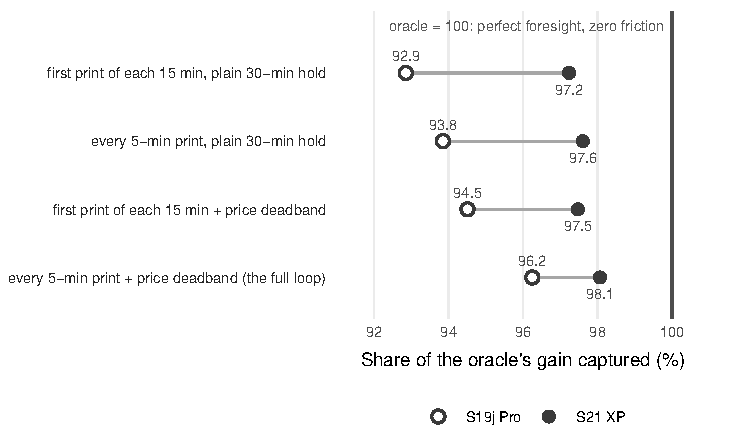
\includegraphics[width=\textwidth]{images/oracle_benchmark}
  \caption{
    Share of the oracle's gain captured by four real configurations at LZ\_WEST, out of sample, for the two fleets of Chapter~4; the gain is profit above running at stock power without ever pausing. The fast feed alone and the price deadband alone each buy little; together they capture 98.1~percent (S21~XP) and 96.2~percent (S19j~Pro) of what perfect foresight gains. Settled on the 15-minute settlement point price, with power curves from the 2026-Q2 fleet data. % fig-src: analysis/figures/fig_ch5_oracle_benchmark.R, which reads analysis/ch5-backtest/output/trend_study/mixed_basis.csv (window TEST-2025-26, zone LZ_WEST, deadband 10 percent of default power; pct_of_s1 98.0661 and 96.2485) and prints the window: 154,975 paired 5-minute intervals, 2025-01-01T00:00Z to 2026-06-23T04:55Z (538 days, to June 22, 2026 Central), out of sample for the price deadband's width, set on 2024; backstop constants: analysis/ch5-backtest/README.md and papo_sim.py provenance note. Billed on ERCOT MIS 13061 settlement point prices, decided on the NP6-788 five-minute prints. The engine runs the 2026-Q2 fleet telemetry curves Figure 5.1 draws, with the modulation floors of telemetry_miner.py modulation_floor: 1,200 W, the S19j Pro's best-efficiency point, and 2,774 W, the S21 XP's Braiins OS default minimum (98.1805 for the S21 XP on its 2,200 W best point, the floor until 2026-09-26). Was 97.6/94.8 on 136,783 intervals to April 2026, from a legacy price cache with a corrupted row
  }
  \label{fig:oracle-benchmark}
\end{figure}

At LZ\_WEST the full loop, five-minute feed plus price deadband plus backstop, captures 95 to 98~percent of what perfect foresight would gain on the newer fleet and 93 to 96~percent on the older one, the lower figures in 2024 and the higher out of sample. % src: analysis/ch5-backtest/output/trend_study/mixed_basis.csv, zone LZ_WEST only, variant decide-5 +deadband10, pct_of_s1 across both windows: S21 XP 95.11 (tune 2024) and 98.07 (test 2025-26), S19j Pro 92.80 and 96.25. The four configurations of Figure 5.5 fall between 88.43 and 98.07 in the two windows
The result is out of sample for only one setting, the price deadband's width, which was set on 2024's prices. The backstop's settings come from an earlier Braiins study whose price record ran from December 2023 to June 2026, and the loop's design itself, deciding on the last print every five minutes under a 30-minute hold, from earlier Braiins backtests on prices that overlap this window. Choosing the backstop's settings on 2024 alone instead moves the out-of-sample result by less than half a point; the design itself was not re-chosen that way. % src: analysis/ch5-backtest/papo_sim.py, provenance note above K_TRIP, and README.md "Provenance of the constants": K_TRIP, RESTART_BAND and DWELL_S (with the runtimes and the cycle budget) come from an earlier Braiins backstop study whose grid search ran on LZ_WEST five-minute prints from 2023-12-11 to 2026-06-23; the price deadband's width, 10% of stock power, is the only setting chosen on TUNE-2024; the loop's design (persistence every five minutes, the 30-minute hold) comes from earlier Braiins work whose backtests overlap TEST-2025-26; capture_anatomy.py console "RETUNE TUNE-2024 pick" (18 settings, K_TRIP 5/10/20 x RESTART_BAND 0/0.05/0.10 x DWELL 15/30 min, best TUNE-2024 capture of the full loop): S21 XP picks K_TRIP 20, band 0.05, dwell 15 (TUNE-2024 95.66 against the printed setting's 95.11, rank 6 of 18), TEST-2025-26 97.86 against 98.07, -0.21 points; S19j Pro picks the printed setting (rank 1), +0.00; "RETUNE all 18 settings on TEST-2025-26, minus the printed setting" -0.86 to +0.05 and -1.16 to +0.29, so "less than half a point" is the 2024 pick's, not every setting's; nothing in the kit re-selects the loop's design on TUNE-2024 alone (papo_sim.py note, README.md), hence "not re-chosen that way"
A strategy with no forecast, no vendor data, and hardware-friendly actuation leaves single-digit percent on the table against perfect foresight. The run-or-pause call is rarely in doubt: in 2025, about 86 percent of LZ\_WEST's five-minute intervals sat below even the stock S19j~Pro's breakeven, where both fleets should run. % src: analysis/checks/ch5_oracle_check.R on analysis/data/ercot_spp_rtm5_lzwest.csv.gz filtered to 2025: 86.5% of 2025 LZ_WEST 5-min intervals below the stock S19j Pro breakeven at the 2025-mean hashprice; below it stock power makes money on both fleets, so the oracle runs (the S21 XP's breakevens are higher: papo_sim.py check_breakevens, 148/144 against 77/65 $/MWh at best point / stock, $44.31/PH/day); ch5_oracle_check.R's oracle pauses at stock power only and decides and bills on the same five-minute print, so its 94.1% for a 1-interval-lag pause-only rule (99.1% of that oracle's profit, always-on 84.3%) is a share of a smaller, pause-only gain, not Figure 5.5's yardstick; against Figure 5.5's oracle, which also moves the power target, pausing alone at stock power takes 22 and 65% (analysis/ch5-backtest/baselines_study.py), as the next paragraph prints
The oracle still pulls ahead in those intervals, through the power target and through how soon the loop resumes after a pause, but the price level persists, so the target the last print points to is usually the one the oracle would have set. % src: analysis/ch5-backtest/capture_anatomy.py console, TEST-2025-26, "SAME-TARGET steps in which the target computed from print i-1 equals the oracle's" (the profit-optimal power target at the previous print, or a pause where even that loses money, against the oracle's on the step itself; a pause counts as a target): 98.85% (S21 XP) and 88.37% (S19j Pro), 99.02 and 88.32 over the oracle's running steps only (2024 98.79 and 89.96); "SAME-TARGET steps at or below the stock S19j Pro breakeven", the counterpart over the whole TEST-2025-26 window, on Figure 5.5's settlement point price, of the 2025 86 percent above: 86.06% of steps, holding 71.63% and 25.77% of the oracle's gain and 16.37% and 38.28% of the full loop's shortfall, the loop paused in 47 and 511 of them, still waiting out the backstop's resume rule
Pausing is where a loop that reacts one print late should lose most, and counted interval by interval it does. Out of sample it is paused in only 79 and 67~percent of the intervals in which the oracle pauses, on the S21~XP and the S19j~Pro. % src: analysis/ch5-backtest/capture_anatomy.py console, TEST-2025-26, "RECON oracle-pause steps in which the full loop is also paused, by count": 78.53% (2,297 of 2,925, S21 XP) and 67.29% (9,033 of 13,424, S19j Pro); 2024 67.20 and 60.10; the oracle pauses in 1.89% and 8.66% of the window's five-minute steps ("RECON oracle pauses in ... steps")
In dollars, though, it recovers 96 and 97~percent of what the oracle's pausing earns. The intervals it misses hold only 5 and 11~percent of that value, and through them the S19j~Pro still turns down, mostly to its floor, which wins back three-quarters of what they are worth. % src: capture_anatomy.py console, TEST-2025-26, "RECON the full loop's recovery of the pause class's gain, in dollars": 96.34% and 97.19% (2024 91.66 and 94.33) of the pause class, the oracle-paused steps, which hold 24.26% and 69.36% of the oracle's gain; of which by being paused 95.45 and 88.57, the rest, net, by running below stock power through those steps, mostly at the floor ("RECON the rest of that recovery ... by applied target": floor +0.58 and +6.47, other targets below stock +0.39 and +2.17, stock power and above -0.10 and -0.02); the steps the loop misses hold 100 - 95.45 = 4.55% and 100 - 88.57 = 11.43% of the pause class's gain, and running through them wins back 96.34 - 95.45 = 0.88 and 97.19 - 88.57 = 8.62, so 8.62 / 11.43 = 75% on the S19j Pro, the floor 6.47 of the 8.62 (0.88 / 4.55 = 19% on the S21 XP); in 2024 the missed steps hold 8.76% and 13.42%, and the S19j Pro wins back 7.75 of its 13.42, 58%
Episodes of more than three hours above breakeven hold about four-fifths of that value, and the loop recovers 99~percent of it. The episodes it handles worst last an hour or less; they are seven in ten of all episodes but hold under a tenth of the value. % src: capture_anatomy.py console, TEST-2025-26, "RECON episodes" (runs of contiguous oracle-paused steps; 155 and 798 episodes): longer than 3 h 14.2% and 10.9% of the episodes, 83.6% and 79.3% of the pause class's gain, recovered at 99.4% and 99.3%; 1 to 3 h 16.8% and 17.3%, 10.1% and 12.1% of the gain, 92.8% and 92.5%; 1 h or less 69.0% and 71.8% of the episodes, 6.3% and 8.6% of the gain, recovered at 61.6% and 84.2%, the lowest; out of sample only: in 2024 episodes over 3 h hold 33.0% and 42.6% of the gain
Leaps far past breakeven usually start falling back at once. LZ\_WEST's price jumped \$100 or more in a single print 555 times from 2024 to mid-2026, about once every 1.6 days, and seven times in ten the very next print was lower. The backstop caps how long any of them can hurt. % src: analysis/checks/ch5_price_autocorrelation.py, first two console lines, LZ_WEST five-minute prints 2024-01-01..2026-06-22 Central (904 days): after rises of $100 or more n=555 (one per 1.6 days), next print lower 69% of the time; after falls of $100 or more it kept falling 71% of the time (one-sided reversion, as line 43 says)

Two baselines give the loop's capture its scale. Never pausing at stock power already earns 90 percent of the oracle's profit on the S21~XP and 75 percent on the S19j~Pro, out of sample and before pool fees, the Braiins~OS development fee (Section~\ref{sec:stack-power-target}) and grid charges. Pausing alone, the backstop at stock power, closes 22 and 65 percent of the remaining gap, and even perfect foresight at stock power, the strike of Chapter~\ref{ch:buying}, would close only 24 and 73 percent. % src: analysis/ch5-backtest/baselines_study.py (output/trend_study/baselines.csv), TEST-2025-26, LZ_WEST, 154,975 paired intervals, Figure 5.5's engine and billing: S0 / S1 profit per machine 5,121.33 / 5,681.21 = 90.1% (S21 XP) and 1,090.76 / 1,458.60 = 74.8% (S19j Pro); both are gross: papo_sim.py and telemetry_miner.py profit() is A*H(p) - B*p, the day's hashprice on the hashrate less the settlement point price on the power, with no pool fee, no Braiins OS development fee (defined in chapter 9 sec:stack-power-target) and no grid charge; backstop alone at stock (floor = ceiling = stock power, stock breakeven, papo_sim.py backstop constants) 22.30% and 65.32% of S1's gain, 0.18 and 0.69 pauses a day; S1 at stock 24.28% and 72.52%; the stock oracle is chapter 6's strike rule on each day's hashprice: over calendar 2025 it is worth $17,636 and $48,945 per MW-year of stock draw, against fig_ch6_strike.R's $17,280 and $49,116 (asserted within 2.5%); on/off at every print at stock, no hold, minimum runtime or cycle budget, 23.39% and 70.40% at 1.3 and 8.1 switches a day; TUNE-2024: always-on 90.7% and 84.7%, backstop alone 14.15% and 47.30%, stock oracle 18.72% and 56.86%; S0, S1 and full-loop rows asserted equal to mixed_basis.csv
The rest is the curve: on the S21~XP almost all of it is running above stock power in cheap intervals, which a site can do only where its connection has room (Section~\ref{sec:stack-power-target}). % src: baselines_study.py TEST-2025-26 LZ_WEST: full loop with its ceiling held at stock 22.65% (S21 XP) and 75.30% (S19j Pro) (console row "full loop, ceiling at stock"; 22.02% and 74.92% before the 2026-10-03 telemetry_miner.scan_powers fix, on the 10 W grid that could not reach 3,645 or 3,068 W; 2024 14.16% and 53.73%), with its floor raised to stock 97.52% and 86.27%, full loop 98.07% and 96.25%; chapter-9.tex sec:stack-power-target (the connection binds: the S21 XP pins at its ceiling and the S19j Pro is held below stock under a 67.13 MW connection)
Given that room, a fixed power target at the S21~XP's 3,990~W ceiling, with the same backstop and no price-following at all, already captures 97.6~percent, so the newer fleet's score mostly grades a setting, not the reflex. On the S19j~Pro a fixed target at its own 3,420~W ceiling captures only 77~percent, and the reflex lifts it to 96. % src: analysis/ch5-backtest/baselines_study.py console row "ceiling + backstop" (output/trend_study/baselines.csv), TEST-2025-26 LZ_WEST: every machine fixed at its power ceiling, 3,990 W (S21 XP) and 3,420 W (S19j Pro), never moved (papo_sim.py simulate(fixed_power=p_max)), paused only by the loop's own backstop at the curve's best-point breakeven, 97.6069% and 77.3556% of the oracle's gain against the full loop's 98.07% and 96.25% (2024 94.93% and 82.70% against 95.11% and 92.80%); with the backstop at the ceiling point's own breakeven instead ("ceiling + backstop (own breakeven)") 97.6172% and 83.1285% (2024 94.867% and 84.5972%)

Call the weakest configuration of Figure~\ref{fig:oracle-benchmark} the naive design: one five-minute print every fifteen minutes (the first of each settlement interval), each power target held at least thirty minutes, the same backstop, and no price deadband. Out of sample at LZ\_WEST, at each day's own hashprice, which averaged about \$0.045 per terahash-day, the full loop earns about \$3,200 a year more than the naive design per thousand S21 XPs, and about \$8,500 more per thousand S19j Pros, some \$900 and \$2,800 a year per megawatt of stock draw. The 30-minute hold alone cuts the S19j~Pro's target moves to under half of retargeting on every print, 13 a day against 32, and the price deadband wins back nearly all of the value the hold gave up, 97 percent of it, with about four-fifths as many moves as retargeting on every print. % src: analysis/ch5-backtest/naive_gap.py (output/trend_study/naive_gap.csv), TEST-2025-26, LZ_WEST, 154,975 paired intervals, 538.2 days: naive design = decide-15 S14, the weakest of Figure 5.5's four out of sample on both fleets (capture 97.23 and 92.85; the hold is a minimum dwell of 1,800 s); full loop = decide-5 +deadband10; full_minus_variant $4.66 (S21 XP) and $12.49 (S19j Pro) per machine, usd_per_year_per_1000 3,158 and 8,469, usd_per_mw_year 866 and 2,760 (3,158 / 3.645 MW and 8,469 / 3.068 MW of stock draw); hashprice console line: the kit's hashprice_daily.csv averages $45.41/PH/day ($0.0454/TH/day) over the paired intervals, the book's Braiins Insights series (analysis/data/hashprice_daily.csv) $45.46 on the same intervals, no day of the window more than $3.77/PH/day apart (2025-11-13 to 15 are absent from the kit's file and carried from the day before) (TUNE-2024 120 and 12,485; against the fast-feed plain hold decide-5 S14, 1,750 and 5,984; the S21 XP's 3,950 was on its 2,200 W best-point floor, until 2026-09-26); S19j Pro changes_day decide-5 S14 13.4, decide-5 every print 32.0, full loop 26.3, 26.3/32.0 = 82%; console fast-feed line: the price deadband wins back 97.3% (S19j Pro) and 98.5% (S21 XP) of what the plain hold gives up against every-print retargeting, which earns 164 and 27 dollars a year per 1,000 more than the full loop; rows shared with mixed_basis.csv asserted equal; the naive design's slow feed is the print stamped at the start of each 15-minute settlement interval, carried for its three steps (mixed_basis_study.py coarsen(), t % 900 == 0), not the settlement point price
Notice who benefits most: the S19j~Pro gains more from every rule than the S21~XP does. That is Chapter~4's operating leverage again, seen from the control room; the closer a machine lives to its breakeven, the more each percentage point of price discipline is worth. The marginal machine needs the reflex most.

Every capture in this chapter charges nothing for a move; the backtest applies each new power target at once, at full efficiency. % src: analysis/ch5-backtest/papo_sim.py simulate() defaults move_loss_s=0 and first_visit_s=0, which every capture in this chapter was computed with: once the hold or the price deadband allows it, the new target applies within the interval and profit is booked at full curve efficiency (README.md, The engine)
Because each target is tuned once and later visits reuse its saved profile, leaving that out costs little. Even three hours of settling on each target's first visit takes under a point off either fleet's capture out of sample. % src: analysis/ch5-backtest/capture_anatomy.py console, TEST-2025-26, "MOVES saved-profile model" (simulate(first_visit_s=...): zero hashing at full draw the first time in a run the loop applies each of its 4 and 8 targets, later visits free): full loop at 10,800 s per first visit 97.17% (S21 XP) and 95.39% (S19j Pro) against 98.07% and 96.25%, -0.90 and -0.86 points; at 600 s 97.99% and 96.18%; 2024 at 10,800 s 93.32% and 90.44% against 95.11% and 92.80%, hence "out of sample"
A cost per move would matter more. Every second of hashing lost per move takes about 0.2 points off the S19j~Pro's capture and about 0.03 off the S21~XP's; the S19j~Pro moves its target about 27 times a day, counting resumes, and the S21~XP under three times. At about 26 seconds a move, the price deadband would stop paying for its extra moves on the S19j~Pro. % src: analysis/ch5-backtest/capture_anatomy.py console, TEST-2025-26, "MOVES decide-5 +deadband10" (simulate(move_loss_s=...): every physical power-target change, a move the hold or the price deadband allows or the target set at a backstop resume, costs that many seconds of hashing with the power still billed): 26.85 physical moves a day (26.34 + 0.51 resumes, S19j Pro) and 2.59 (2.42 + 0.17, S21 XP); 0.1882 and 0.0345 capture points per second (2024 0.2000 and 0.0356); capture at 30 s 90.60% and 97.03%; "MOVES full loop stops beating decide-5 S14 at" 26.3 s (S19j Pro; 2024 29.5 s), the plain hold on the same five-minute feed, the full loop without its price deadband (43.1 s on the S21 XP); against the naive design ("stops beating decide-15 S14 at") 33.4 s and 55.2 s; the per-move cost is a sensitivity, not a measured firmware figure

The design work behind this chapter is Braiins' own, and it is published here for the first time. Everything else in this paragraph you can rerun yourself from the companion repository. It recomputes the ladder above on ERCOT's own published prices and on the same fleet curves Figure~\ref{fig:efficiency-curves} draws. It shows the price deadband beating the plain hold in all sixteen zone-and-fleet combinations, in 2024 and again in January 2025 through June 2026, at each of the three widths tried from 10 to 25~percent. So the result does not hang on where the width was set. At the fourth, 40~percent, it never fires on the S21~XP, whose whole power range is narrower than that, and there it only ties the plain hold. And it checks the optimizer that picks each power target against an exhaustive search over every operating point between each curve's floor and ceiling. The check uses about 250,000 ERCOT price observations: a sample of 200,000 positive prices plus all 50,000 zero or negative prices in LZ\_WEST's five-minute prints and the eight load zones' 15-minute settlement prices, from January 2024 through June 2026. The two methods pick the same target every time. % src: ladder: analysis/ch5-backtest/mixed_basis_study.py (output/trend_study/mixed_basis.csv); price deadband: analysis/ch5-backtest/multizone_study.py --all-zones summary (DEADBANDS 0.10, 0.15, 0.25, 0.40; output/trend_study/multizone_rtm15.csv): uplift above the plain hold in 16/16 cells at 10, 15 and 25% in TUNE-2024 and in TEST-2025-26, and in 8/16 at 40%, where the 8 S21 XP cells equal the plain hold exactly (delta_vs_s14 0.0: 40% of 3,645 W is 1,458 W, more than the 1,216 W between the 2,774 W floor and the 3,990 W ceiling, so the deadband cannot fire; 16/16 at all four widths on the 2,200 W best-point floor, until 2026-09-26), pause count unchanged; re-run 2026-09-26 on the S21 XP's 2,774 W floor; optimizer: analysis/ch5-backtest/optimizer_bruteforce_check.py summary (output/trend_study/optimizer_bruteforce.csv): 250,214 real prices 2024-01-01 to 2026-06-24 UTC, 124,745 LZ_WEST NP6-788 prints and 125,469 MIS 13061 settlement point prices over 8 zones, a seeded sample of 100,000 positive prices per series plus every price at or below zero in both series, 50,214 of them (low -228.75 $/MWh), so the sample over-weights them; candidates are the measured points between each curve's floor and ceiling plus the interpolated ends of the range (the 3,420 and 3,990 W ceilings and the S21 XP's 2,774 W floor); same power target in 500,428 of 500,428 choices over both fleets, largest shortfall 0.00 $/machine-hour, 0 run-or-pause disagreements; a deliberately broken 50 W scan fails the same check; "published here for the first time" per author request 2026-08-27
None of this is a field result. The loop's numbers are backtests on ERCOT's published prices and fleet-average curves, so that a reader can rerun them; the book's field evidence of what pausing earns is what Riot, a listed miner, reports (Chapters~2, 3 and~6). % src: analysis/ch5-backtest (mixed_basis_study.py, baselines_study.py and naive_gap.py on ERCOT MIS 13061 settlement point prices and NP6-788 LZ_WEST prints, with the fleet-average curves of analysis/data/miner_efficiency_telemetry_2026q2.csv); the kit replays no site's own record; field evidence: chapter-2.tex:106 (Riot2024Jan, Riot2025Jan: curtailment and demand-response credits), chapter-3.tex:132 (August 2023 resale and demand response), chapter-6.tex:83 and :136 (riot10k2025, riot10k2024 power curtailment credits); ERCOT's own measurements of the mining response, chapter-3.tex:124 (about 4,100 MW of Winter Storm Fern curtailment credited to miners) and chapter-8.tex:88 (about 3,150 MW cut on August 18, 2025), are megawatts, not what the pauses earned

Price Adapt in Braiins Manager, the fleet software I work on at Braiins, implements the loop. It uses electricity prices, hashprice and the machine's efficiency curve to choose the most profitable power target, or a pause when running does not pay. Braiins~OS autotuning puts the chosen target into practice by adjusting each chip's voltage and frequency \autocite{braiinsacademypriceadapt,braiinsacademyautotuning}. % src: braiinsacademypriceadapt, read 2026-09-25: Price Adapt uses Day-Ahead Market (DAM) pricing and a daily planning cycle builds the next day's plan; for each hour it evaluates each miner model's efficiency curve against energy price and hashprice and selects the power setting with the highest hourly net profit; if no setting is profitable the miner is curtailed (paused) for that hour; power-target changes on supported Braiins OS models, pause and resume only on stock firmware; profile field Tolerance (USD/MWh) shifts the profitability threshold for both curtailment and power-target decisions; ERCOT and PJM day-ahead prices; currently under active development
% Historical provenance (detail removed from prose on 2026-10-02): Braiins Academy Continuous Tuning page, read 2026-09-25 (page titled Continuous Tuning (beta); an advanced autotuning mode, enabled in Advanced Settings, that replaces the one-off tune; every tuning cycle, approximately 5 minutes, recalculates frequencies and voltages for current conditions; the About page says every few minutes); Braiins OS release notes, release 26.04 dated April 15, 2026: continuous tuner in official beta, still beta through 26.09.1 of September 24, 2026; how it reaches a new power target is stated on no public Braiins page checked, so nothing is printed about it

And with that, the reflex is done. Capture in the nineties means the remaining money is not in better reflexes. It is in two places this loop cannot reach: buying the electricity better in the first place, which is Chapter~6's contract menu and strike price, and getting paid for the readiness itself, which is what ERCOT's ancillary services buy and Chapters~7 through 9 price. The machine can now flex. The rest of this book is about selling it.
